%        File: hw2.tex
%     Created: Sun Oct 2 05:00 PM 2013 E
% Last Change: Sun Oct 2 05:00 PM 2013 E
%
\documentclass[a4paper]{report}

\title{HW 4}
\author{Delos Chang}
\date{}

\usepackage{amsmath, amsthm, amssymb, fancyhdr, tikz, algorithmicx, algpseudocode, algorithm}
\usepackage{mathtools}
\DeclarePairedDelimiter{\floor}{\lfloor}{\rfloor}
\usetikzlibrary{arrows}
\newcommand{\justif}[2]{&{#1}&\text{#2}}
\renewcommand{\algorithmicforall}{\textbf{for each}}

\pagestyle{fancy}
\rhead{HW 4:  Delos Chang (help from Prof.)}
\begin{document}
    Questions:
      \#3 Pre and post conditions for 
  \begin{enumerate}
    %&=& &=& &=& &=& &=& &=& &=& &=& &=& &=& &=& &=& &=& &=& &=& =
    % Question 1 
    %&=& &=& &=& &=& &=& &=& &=& &=& &=& &=& &=& &=& &=& &=& &=& =
    \item 


    %&=& &=& &=& &=& &=& &=& &=& &=& &=& &=& &=& &=& &=& &=& &=& =
    % Question 2 
    %&=& &=& &=& &=& &=& &=& &=& &=& &=& &=& &=& &=& &=& &=& &=& =
    \par
    \bigskip

    \item 
      {\bf Overview:}

      1. Given graph G=(V,E), run SCC(G), as defined in class, 
      forming the component graph $G^{SCC} = (V^{SCC}, E^{SCC})$, a DAG. 

      2. Let $k$ denote the number of vertices in $V^{SCC}$. Run topological sort on the component graph $G^{SCC}$, 
      which will produce a linear order of vertices $V_{chain} = \{v_{0}, v_{1}, v_{2} \dots v_{k}\}$. 

      3. Check that this linear ordering of vertices is a chain. 
      In other words, check that from $i=0$ to $i=k-1$, $v_{i},v_{i+1} \in V_{chain}$ (assuming $v_{0}$ is the first vertex
      , the edge $(v_{i},v_{i+1}) \in E^{SCC}$.
      Note that $V_{chain}$ is not necessarily a linearly ordered chain.

      If edges $(v_{0}, v_{1}), (v_{1},v_{2}),\dots,(v_{k-1},v_{k}) \in E^{SCC}$, then $G$ is a semi-connected graph.
      If any of the aforementioned edges do not exist in $E^{SCC}$, then $G$ is not a semi-connected graph. 

      {\bf Pseudocode:}

      \begin{algorithmic}[1]
        \Function{SemiConnected}{$G(V,E)$}

        \State $G^{SCC}(V^{SCC},E^{SCC})$ = SCC($G=(V,E)$)
        \Comment Form component graph $G^{SCC}$

        \State $V_{chain}$ = TopSort($G^{SCC}$)
        \Comment $V_{chain}$ contains list returned by top sort

        \State $i=0$
        \Comment Check $V_{chain}$ if it contains linearly chained edges
        \While{$i < |V_{chain}|$}
          \If {$(v_{i},v_{i+1}) \not\in E^{SCC}$}
            \State return false
          \EndIf
          \State i++

        \EndWhile
        \State return true
      \EndFunction
    \end{algorithmic}

      {\bf Correctness:}
      All vertices in each strongly connected component are mutually reachable. 
      Thus, by definition, for all pairs of vertices $u$,$v$ in each strongly connected component graph, $u \leadsto v$ and $v \leadsto u$. 
      In other words, strongly connected components are semi-connected graphs. 
      These mutually reachable vertices are represented as one vertex in $V^{SCC}$. 

      Hence, if $G^{SCC}$ is semi-connected, then $G$ is semi-connected. 
      
      Let a linearly ordered chain be a set of vertices such that in $V_{chain}$ with $k$ SCCs, the
      edges $(v_{0}, v_{1}), (v_{1},v_{2}),\dots,(v_{k-1},v_{k}) \in E^{SCC}$.

      {\it Claim 1:} If there is a linearly ordered chain in $G^{SCC}$, $TopSort(G^{SCC})$ returns the linearly ordered chain. 

      A topological sort returns a linear ordering of all its vertices such that if $G$ contains an edge $(u,v)$, then $u$
      appears before $v$ in the ordering. Hence, it is vacuously true that because topological sort outputs vertices with respect 
      to its order in the edges, topological sort must return a linearly ordered chain if there is one. 

      {\it Claim 2:} $G^{SCC}$ is semi-connected iff $V_{chain}$ is a linearly ordered chain. 

      {\it Subclaim 1:} $G^{SCC}$ is semi-connected if $V_{chain}$ is a linearly ordered chain. 

      Consider $G^{SCC}=(V^{SCC}, E^{SCC})$ and that $V_{chain}$ is a linearly ordered chain generated by the topological sort on $G^{SCC}$. 

      Hence, between any two arbitrary vertices $u$,$v \in V^{SCC}$, either $u$ is a vertex before $v$ in the linearly ordered chain $V_{chain}$ or
      $v$ is a vertex before $u$. In the former case, $u \leadsto v$ through some chain of edges found by following the edges in 
      $V_{chain}$. In the latter case $v \leadsto u$ through some chain of edges. 

      Thus, because $u$ and $v$ can be arbitrary vertices in $V^{SCC}$, $G^{SCC}$ is semi-connected. 


      {\it Subclaim 2:} $G^{SCC}$ is not semi-connected if $V_{chain}$ is not a linearly ordered chain. 

      Consider $V_{chain}$ is not a linearly ordered chain. Then some two consecutive vertices $v_{i}$ and 
      $v_{i+1} \in V_{chain}$ but $(v_{i}, v_{i+1}) \not\in E^{SCC}$. 

      Either $v_{i}$ has outgoing edges or it doesn't. If $v_{i}$ has no outgoing edges, then there cannot be any path from
      $v_{i}$ to $v_{i+1}$, by definition. 

      If $v_{i}$ has outgoing edges, because of the property of topological sort in producing a linear ordering, edges from $v_{i}$ to 
      $v_{n}$ where $n > i+1$. Because each vertex $\in V^{SCC}$, no two vertices in $V^{SCC}$ are mutually reachable. Otherwise, 
      they would not be the maximal set, by definition of SCC. Furthermore, because of the linear ordering of topological sort, 
      there can be no path from any $v_{n}$ to $v_{i+1}$ ($v_{i+1}$ precedes $v_{n}$). 
      
      Hence, there can be no path from $v_{i}$ to $v_{i+1}$.

      Now, we show that no paths exist from $v_{i+1}$ to $v_{i}$.
      Because $v_{i}$ precedes $v_{i+1}$ and no two vertices in $V^{SCC}$ are mutually reachable (otherwise they would be in the same
      SCC), by top sort, there can be no paths from $v_{i+1}$ to $v_{i}$. 

      Hence, we have Subclaim 2 because no path exists from $v_{i+1}$ to $v_{i}$ or $v_{i}$ to $v_{i+1}$. 

      With Subclaim 1 and Subclaim 2, we have Claim 2. 


      {\bf Time Complexity:}
      
      Running SCC using DFS on $G$, then DFS on $G^{T}$ (transpose graph) as defined in class takes $\Theta(V+E)$.
      Forming the component graph takes $O(V+E)$. 
      Running Topological Sort on $G^{SCC}$ with DFS in reducing finishing times as defined in class takes $O(V+E)$ because.
      $G^{SCC}$ has at most $|V|$ vertices and $|E|$ edges. 
      To check the linearly ordered chain, the algorithm will check each vertex $v_{i}$ in $G^{SCC}$'s adjacency list to check for
      $(v_{i}, v_{i+1})$. Thus, the adjacency list is checked exactly once. Thus, $O(V+E)$.

      Hence, the time complexity of this algorithm is $\Theta(V+E)$.


    %&=& &=& &=& &=& &=& &=& &=& &=& &=& &=& &=& &=& &=& &=& &=& =
    % Question 3 
    %&=& &=& &=& &=& &=& &=& &=& &=& &=& &=& &=& &=& &=& &=& &=& =
    \par
    \pagebreak
    \bigskip
    \setcounter{equation}{0}

    \item
      We modify the Mergesort algorithm on page 31 and 34.
      
      Given an array $A$ of ints size $n$, initialize the following pseudocode with $inversions(A, n)$: 

      {\bf Pseudocode:}
      \begin{algorithmic}[1]
        \Function{inversions}{$A, n$}
          \State $count = countInv(A, 1, n)$
          \State return $count$
        \EndFunction
      \end{algorithmic}

      {\it Pre-Condition:}

       - $n \geq 1$

      {\it Post-Condition:}

        - $count$ is the number of inversions in  $A[1 \dots n]$

        - $A[1\dots n]$ is a sorted permutation of the original array, $A'[1\dots n]$.

      {\bf Pseudocode:}
      \begin{algorithmic}[1]
        \Function{countInv}{$A, p, r$}
          \State $count = 0$
          \If {$p < r$}
            \State $q = \floor{(p+r) / 2}$
            \State $count +=$ countInv($A, p, q$)
            \State $count +=$ countInv($A, (q+1), r$)
            \State $count +=$ main($A, p, q, r$)
          \EndIf
          \State return $count$
        \EndFunction
      \end{algorithmic}

      {\it Pre-Condition:}

       - $p \leq r$

      {\it Post-Condition:}

        - $A[p\dots r]$ is a sorted permutation of the original array, $A'[p \dots r]$

        - for all $(m < p) \wedge (m > r), A[m] = A'[m]$

        - $count$ is the number of inversions in the {\it new} sorted permutation $A[p \dots r]$

      



      {\bf Pseudocode:}
      \begin{algorithmic}[1]
        \Function{main}{$A, p:$ first index of 1st seg, $q$:ending index of 1st seg, $r$:ending index of 2nd seg}
          \State $n_{1} = q - p + 1$
          \Comment Checking length of subarrays
          \State $n_{2} = r - q$
          \State let $L[1\dots n_{1} + 1]$ and $R[1\dots n_2 + 1]$ be new arrays
          \ForAll{$i = 1$ to $n_1$}
            \State $L[i]  = A[p + i - 1]$
          \EndFor
          \ForAll{$j = 1$ to $n_2$}
            \State $R[j] = A[q + j]$
          \EndFor

          \Comment add sentinel to know when to stop
          \State $L[n_1 + 1] = \infty$
          \State $R[n_2 + 1] = \infty$

          \State $i = 1$
          \State $j = 1$

          \State $checked = false$
          \State $count = 0$

          \ForAll{$k = p$ to $r$}
            \If {$L[i] > R[j] $ and $checked = false$}
              \State $checked = true$
              \State $count += n_1 - i + 1$
            \EndIf

            \If {$L[i] \leq R[j]$}
              \State $A[k] = L[i]$
              \State $i++$
            \Else 
              \State $A[k] = R[j]$
              \State $j++$
              \State $checked = false$
            \EndIf
          \EndFor
          \State return count
        \EndFunction
      \end{algorithmic}

      {\it Pre-Condition:}

        - $p \leq q \leq r \wedge$ $A[p\dots q]$ is sorted $\wedge$ $A[q+1\dots r]$ is sorted 

      {\it Post-Condition:}

        - $A[p\dots r]$ is a sorted permutation of $A'[p \dots r]$

        - for all $(m < p) \wedge (m > r), A[m] = A'[m]$

        - $count$ is the number of inversions in the {\it new} sorted permutation $A[p \dots r]$



      
     {\bf Time Complexity}
      
        - Merge sort's time complexity is $\Theta(n \cdot log n)$. To modify the original Merge Sort, we added lines that only
        take constant amount of time (assignments and constant time if statement checks):

        - In $countInv$, the initializations and assignments of $count$ take $\Theta(1)$ time.

        - Assignment on line (15) and (16) of $main$ take $\Theta(1)$ time.

        - on lines (18) - (21) of $main$, the $if$ statement checks for an inversion. The checks and assignments take $\Theta(1)$.

        Hence, the time complexity for this algorithm is the same as merge sort: $\Theta(n \cdot log n)$.
        





    %&=& &=& &=& &=& &=& &=& &=& &=& &=& &=& &=& &=& &=& &=& &=& =
    % Question 4 
    %&=& &=& &=& &=& &=& &=& &=& &=& &=& &=& &=& &=& &=& &=& &=& =
    \par
    \bigskip
    \pagebreak
    \setcounter{equation}{0}
    
    \item 



    
    %&=& &=& &=& &=& &=& &=& &=& &=& &=& &=& &=& &=& &=& &=& &=& =
    % Question 5 
    %&=& &=& &=& &=& &=& &=& &=& &=& &=& &=& &=& &=& &=& &=& &=& =
    \bigskip
    \setcounter{equation}{0}

    \item 
      % a)

      a) 
      $2^n = o(n!)$:

      Fact: If log $f(n) = o($log $g(n))$, then $f(n) = o(g(n))$. 
      Using this fact, let $f(n) = 2^n$ and $g(n) = n!$. Thus, taking logs of both sides:

      \begin{align}
        log(2^n) = n \cdot log 2 \\
        log(2^n) = n \\
        log(n!) = \theta(n \cdot log n) 
      \end{align}

      Because $\theta(n \cdot$ log $n) = \omega(n)$, it follows that $2^n = o(n!)$.

      \bigskip
      % b)
      b) $5^{log n} = o(6^{log n})$:
      
      Fact: $a^{log_{b} c}$ = $c ^ {log_{b} a} $. Thus:
      \begin{align}
        6^{log n} = n^{log 6} \\
        5^{log n} = n^{log 5} 
      \end{align}

      $Fact: n = o(n^2)$. Similarly, because $log 6 > log 5$, $n^{log 5}$ = $o(n^{log 6})$. 
      Thus, by identity, $5^{log n} = o(6^{log n})$.

      \bigskip
      % c)
      c) None of the above:
      
      The co-domain of a sine function is [-1, 1]. Thus, for all $n$, $n^{-1} \leq n^{sin n} \leq n$.

      Thus, depending on $n$, sometimes $n^{sin n} > \sqrt{n}$, sometimes $n^{sin n} < \sqrt{n}$.
      It follows that there are no positive real constants $n_{0}, c$ such that for {\bf all} $n \geq n_{0}$,  $n^{sin n} \leq c \cdot \sqrt{n}$.
      For every $n_{1}$ where $n_{1}^{sin n_{1}} \leq c \cdot \sqrt{n_{1}}$, there exists a $n_{2}$ where $n_{2} > n_{1}$ and $n_{2}^{sin n_{2}} \geq c \cdot \sqrt{n_{2}}$.
      Thus $n^{sin n} \neq O(\sqrt{n})$, which implies that $n^{sin n} \neq o(\sqrt{n})$.

      For the same reason, there are no positive real constants $n_{0}$, $c$ such that for all $n \geq n_{0}$, 
      $n^{sin n} \geq c \cdot \sqrt{n}$. 
      Thus $n^{sin n} \neq \Omega(\sqrt{n})$, which implies that $n^{sin n} \neq \omega(\sqrt{n})$.

      Hence, none of the above.

      \bigskip
      % d)
      d) 
      $f(n) = O(n^2)$:

      If $f(n) = O(n^2)$, there exist $c > 0$, $n_{0} > 0$, such that for all $n \geq n_{0}$, 
      $f(n) = c \cdot n^2$.

      Consider when $c = 6$ and $n_{0} = 1$:
      
      $$ f(n) \leq 6n^2 \text{ for all } n \geq 1 $$

      For all $n \geq 1 $, $f(n) \leq 5n^2$. Because for $n \geq 1$,
      $5n^2 \leq 6n^2$, $f(n) \leq 6n^2$ for all $n \geq 1$ is true. 

      Thus, by definition of $O$, $f(n) = O(n^2)$. 
      
      $f(n) \neq \Omega(n^2)$ because for any $n_{0}$ such that $f(n_{0}) \geq c \cdot (n_{0})^2$, 
      there exist a $n_{1} > n_{0}$ where $f(n_{1}) \leq c \cdot (n_{1})^2$. 


      \bigskip
      % e)
      e) 
      $(n!)^{n} = o(2^{2^{n}})$:

      Fact: If log $f(n) = o($log $g(n))$, then $f(n) = o(g(n))$. 
      Using this fact, let $f(n) = (n!)^{n}$ and $g(n) = 2^{2^{n}}$. Thus, taking logs of both sides:

      \begin{align}
        log(n!^{n}) = n \cdot log(n!)\\
        log(n!^{n}) = n \cdot \theta(n \cdot log n)\\
        log(n!^{n}) = \theta(n^2 \cdot log n)\\
        log(2^{2^{n}}) = 2^n 
      \end{align}

      $2^n$ drowns $\theta(n^2 \cdot log n)$ because exponential time complexity drowns polynomial
      time complexity.
      Therefore, $\theta(n^2 log n) = o(2^{n})$, it follows from the aforementioned fact that:

      $(n!)^{n} = o(2^{2^{n}})$

    %&=& &=& &=& &=& &=& &=& &=& &=& &=& &=& &=& &=& &=& &=& &=& =
    % Question 6 
    %&=& &=& &=& &=& &=& &=& &=& &=& &=& &=& &=& &=& &=& &=& &=& =
    \pagebreak
    \bigskip
    \setcounter{equation}{0}
    \item We disprove by considering the counterexample where log $f(n) = O($log $g(n))$ but $f(n) \neq O(g(n))$: 
    
      Consider $f(n) = n^3$ and $g(n) = n$. 

      \begin{align}
        log(f(n)) = 3 \cdot log(n)                    &&\text{Taking log of f(n)}\\
        log(g(n)) = log(n)                            &&\text{Taking log of g(n)}\\
        log(f(n)) = O(log(n))                         &&\text{Def of $O$}
      \end{align}

      We have shown the first part of the implication. But it is evident that $n = O(n^3)$.
      Thus, while log $f(n) = O($log $g(n))$, $f(n) \neq O(g(n))$, disproving the statement.

    %&=& &=& &=& &=& &=& &=& &=& &=& &=& &=& &=& &=& &=& &=& &=& =
    % Question 7 
    %&=& &=& &=& &=& &=& &=& &=& &=& &=& &=& &=& &=& &=& &=& &=& =
    \bigskip
    \setcounter{equation}{0}
    \item We disprove the statement by considering a counterexample: 

      Consider $g(n) = 1$ everywhere and $f(n)$ where $f$ is defined as follows: $f(n) = 1$ if $n$ is even; else $f(n) = n^{-1}$.
      Let $c = 1$ and $n_{0} = 1$. Then:

      $f(n) \leq c \cdot g(n)$ for all $n \geq n_{0}$.
      Simplifying: $f(n) \leq 1$ for all $n \geq 1$, which is true because the biggest value $f(n)$ can be is 1.

      Thus, by definition, $f(n) = O(g(n))$.

      Next, we show that $f(n) \neq \Omega(g(n))$.

      Because $f(n) = n^{-1}$ when $n$ is odd, there are infinite n's that dip below any constant infinitely often.
      In other words, as n approaches infinity, $f(n)$ oscillates between 1 and falls below any constant infinitely. 
      Thus, no positive real constant $n_{0}$ exists such that $f(n) \geq c \cdot g(n)$ for all $n \geq n_{0}$.

      Hence, by definition, $f(n) \neq \Omega(g(n))$. 
      
      Finally, we show that $f(n) \neq o(g(n))$.
      For $f(n) = o(g(n))$ to be true, for {\bf any} positive constant $c > 0$, there must exist a constant $n_{0} > 0$ such that
      $0 \leq f(n) < c \cdot g(n)$ for all $n \geq n_{0}$. 

      Consider $c = 0.4$. $g(n) = 1$ everywhere and $f(n) > 0.4 * 1$ infinitely many times as n approaches infinity 
      (when n is even). Thus, there is no $n_{0} > 0 $ such that $0 \leq f(n) < c \cdot g(n)$ for all $n \geq n_{0}$.  
      
      We have shown this condition to fail for $c = 0.4$, $f(n) \neq o(g(n))$.

      Hence, we have disproved the statement.

    %&=& &=& &=& &=& &=& &=& &=& &=& &=& &=& &=& &=& &=& &=& &=& =
    % Question 8 
    %&=& &=& &=& &=& &=& &=& &=& &=& &=& &=& &=& &=& &=& &=& &=& =
    \bigskip
    \setcounter{equation}{0}
    \item 
      Adjacency List Algorithm:

      \begin{align*}
        &\text{transpose(V:vertices, adj:adjacency list)\{} \\
        & \hspace{1cm} \text{for each $v \in V$} \\
        & \hspace{2cm} \text{adjNew[v] $\leftarrow$ nil}  &&\text{//initialize new adj list} \\
        & \hspace{2cm} \text{for each $u \in $ adj[v]} \\
        & \hspace{3cm} \text{adjNew[u].insert(v)} &&\text{//linked list insert method}\\
        & \hspace{1cm} \text{return adjNew} \\
        &\text{\}} \\
      \end{align*}

      The entire algorithm loops through exactly each of the vertices and each of the edges (as represented by the adjacency list) once.

      Setting adjNew[v] to nil takes $\Theta(1)$ time and inserting into a linked list takes $\Theta(1)$ time.

      Thus the time complexity of this algorithm is $O(|V| + |E|)$ where $|V|$ are the number of vertices and $|E|$ are the number of edges.

      \bigskip
      Adjacency Matrix Algorithm:
      \begin{align*}
        &\text{transpose(V:vertices, adj:adjacency matrix)\{} \\
        & \hspace{1cm} \text{for $i \leftarrow 1$ to $|V|$} &&\text{// not zero-indexed}\\
        & \hspace{2cm} \text{for $j \leftarrow 1$ to $|V|$} \\
        & \hspace{3cm} \text{adjNew[j, i] $\leftarrow$ adj[i, j]} &&\text{//swap values around}\\
        & \hspace{1cm} \text{return adjNew} \\
        &\text{\}} \\
      \end{align*}

      The running time is $O(|V|^2)$ because assigning the adjNew indices takes $\Theta(1)$ and for every vertice, we examine all the vertices. 
      The running time is slower than the adjacency list algorithm because we needlessly look at the existence of certain edges. 

    %&=& &=& &=& &=& &=& &=& &=& &=& &=& &=& &=& &=& &=& &=& &=& =
    % Question 9 
    %&=& &=& &=& &=& &=& &=& &=& &=& &=& &=& &=& &=& &=& &=& &=& =
    \bigskip
    \setcounter{equation}{0}
    \item 

      \bigskip
      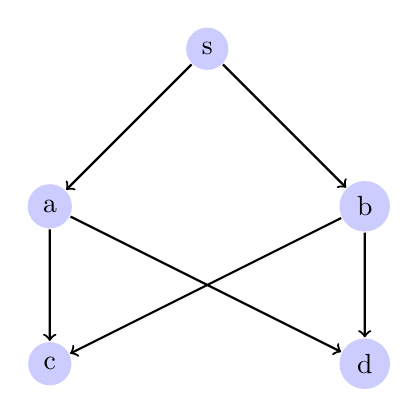
\begin{tikzpicture}
        [scale=.8,->,thick,auto=left,every node/.style={circle,fill=blue!20}]
        \node (n6) at (5,10) {s};
        \node (n4) at (2.5,7.5)  {a};
        \node (n5) at (7.5,7.5)  {b};
        \node (n1) at (2.5,5) {c};
        \node (n2) at (7.5,5)  {d};

        \foreach \from/\to in {n6/n4,n6/n5,n5/n1,n5/n2, n4/n1, n4/n2}
        \draw (\from) -- (\to);
      \end{tikzpicture}

      In this graph $G(V,E)$, the source vertex $s \in V$. 

      The set of tree edges, $E_{\pi}$=\{(s,a),(a,c),(s,b),(b,d)\}. Furthermore, $E_{\pi} \subseteq E$ 
      is such that for each vertex $v \in V$, the unique simple path in the graph $(V,E_{\pi})$ from $s$ to $v$
      is a shortest path in $G$.

      $E_{\pi}$ cannot be produced by running BFS on $G$, no matter how the vertices are ordered in each adjacency list.
      To see why, let $adjList$ be the adjacency list for $G(V,E)$. Suppose BFS starts with $s$ and $adjList[s]$ links $a$ before $b$.
      In this case, BFS would add edges (s,a) and (s,b) to the BFT (breadth-first tree and enqueue $a$ before $b$. Dequeuing $a$,
      BFS would then add edges (a,c) and (a,d) to BFT. Thus (b,d) is never added to BFT.

      If $adjList[s]$ links $b$ before $a$, then following the same process with BFT, (a,c) would never be added. Hence, BFS will never
      add both (a,c) and (b,d) to the BFT as tree edges. Thus, the set of edges $E_{\pi}$ cannot be produced by running BFS on $G$. 

    %&=& &=& &=& &=& &=& &=& &=& &=& &=& &=& &=& &=& &=& &=& &=& =
    % Question 10 
    %&=& &=& &=& &=& &=& &=& &=& &=& &=& &=& &=& &=& &=& &=& &=& =
    \pagebreak
    \bigskip
    \setcounter{equation}{0}
    \item 

      Algorithm:

      Consider a graph $G=(V,E)$ where each vertex is a wrestler and an edge represents a rivalry between two wrestlers.
      Thus, there are $n$ vertices and $r$ edges. If $G$ is bipartite, there will be no odd length cycles. 

      - Initialize an arbitrary source vertex as $good$. Start BFS with this source vertex. \\
      - While running BFS, mark every adjacent node the opposite of its ancestor. E.g.: adjacent vertices of the source vertex 
      will be marked $bad$. \\
      - Repeat BFS with each disconnected graph. \\
      - If we discover an odd length cycle (i.e. $good$ vertex adjacent to $good$ or $bad$ vertex adjacent to $bad$), stop 
      the algorithm because the conflicting edge proves no proper labelling exists. \\
      - If no odd length cycles are discovered (no label conflicts), we have produced a correctly labelled graph of $n$ wrestlers and $r$ edges. \\

      Let $\pi[v]$ indicate the type $"good", "bad", "nil"$ for vertex $v$.
      \begin{align*}
        &\text{main($G=(V,E)$, $s$:source vertex)\{} \\
        & \hspace{1cm} \text{//initialize status:nil for each vertex}\\
        & \hspace{1cm} \text{for each $v \in V$} \\
        & \hspace{1.5cm} \text{$\pi[v] \leftarrow$ nil} \\
        & \hspace{1cm} \text{BFS($G$, $s$)} \\\\
        & \hspace{1cm} \text{//run BFS on any disconnected graphs}\\
        & \hspace{1cm} \text{for each $v \in V$} \\
        & \hspace{1.5cm} \text{if $\pi[v] == nil$}  \\
        & \hspace{2cm} \text{BFS($G$, $v$)}   \\
        &\text{\}} 
      \end{align*}

      \begin{align*}
        &\text{BFS($G=(V,E)$, $s$:source vertex)\{} \\
        & \hspace{1cm} \text{$\pi[s] \leftarrow $ "good"} \\
        & \hspace{1cm} \text{enqueue($Q$,$s$)} \\
        & \hspace{1cm} \text{while $Q$ is not empty} \\
        & \hspace{1.5cm} \text{u = dequeue($Q$)}   \\
        & \hspace{1.5cm} \text{for each $v \in Adj[u]$}   \\
        & \hspace{2cm} \text{if $\pi[v] == nil$}   \\
        & \hspace{2.5cm} \text{if $\pi[u] == $ "good"}   \\
        & \hspace{3cm} \text{$\pi[v] \leftarrow $ "bad"}   \\
        & \hspace{2.5cm} \text{elseif $\pi[u] == $ "bad"}   \\
        & \hspace{3cm} \text{$\pi[v] \leftarrow $ "good"}   \\
        & \hspace{2.5cm} \text{enqueue($Q$,$v$)}   \\
        & \hspace{2cm} \text{elseif $\pi[u] == \pi[v]$ and $u$ != $v$}   \\
        & \hspace{2.5cm} \text{sys.exit()}  &&\text{// exit program: conflict proves odd cycle length} \\
        &\text{\}} 
      \end{align*}

      Each edge is explored at most twice with $\Theta(1)$. The $while$ loop in BFS is done 
      at most $v$ iterations (covering every disconnected graph).

      Thus, the time complexity is $O(|V|+|E|)$

    %&=& &=& &=& &=& &=& &=& &=& &=& &=& &=& &=& &=& &=& &=& &=& =
    % Question 11 
    %&=& &=& &=& &=& &=& &=& &=& &=& &=& &=& &=& &=& &=& &=& &=& =
    \bigskip
    \setcounter{equation}{0}
    \item 
      Consider an adj matrix $A$ that represents graph $G = (V,E)$ i.e. $|V| x |V|$.

      If graph $G$ contains a universal sink, the following algorithm 
      returns the universal sink vertex in time $O(V)$ given adj matrix $A$.

      If graph $G$ does not contain a universal sink, the algorithm returns $false$ in time $O(V)$.

      \begin{align*}
        & \text{main($G=(V,E)$, $A$:adjacency matrix)\{} \\
        & \hspace{1cm} \text{$cand$ = 1} \\
        & \hspace{1cm} \text{for $i \leftarrow 2$ to $|V|$\{ } \\
        & \hspace{1.5cm} \text{if $A[cand][i] == 1$}   \\
        & \hspace{2cm} \text{$cand \leftarrow i$}   \\
        & \hspace{1cm} \text{\}}   \\
        & \hspace{1cm} \text{return(check($cand$))} \\
        &\text{\}} \\
      \end{align*}

      \begin{align*}
        & \text{check($cand$)\{} \\
        & \hspace{1cm} \text{for $i \leftarrow 1$ to $|V|$)\{ } \\
        & \hspace{1.5cm} \text{if $A[cand][i]$ != $0$}   \\
        & \hspace{2cm} \text{return $false$}   \\
        & \hspace{1.5cm} \text{if $i$ != $cand$ and $A[i][cand]$ != $1$}   \\
        & \hspace{2cm} \text{return $false$}   \\
        & \hspace{1cm} \text{\}}   \\
        & \hspace{1cm} \text{return($cand$)} \\
        &\text{\}} \\
      \end{align*}

      The $sink$ function's runtime is $O(|V|)$ because it loops through each vertex to check columns for 0 (excluding $A[cand][cand]$)
      and rows for 1. Each iteration takes $\theta(1)$ time. 
      The $main$ function's runtime is $O(|V|)$ where each iteration also takes $\theta(1)$ time. It never loops through more than $|V|$.

      The $main$ function's loop returns in the $cand$ variable the only vertex in the adjacency matrix which is a $possible$ universal sink. 

      Loop Invariant: $2 \leq i \leq |V| + 1$ $\wedge$ every vertex $1\dots i-1$, excluding $cand$, are not universal sinks.\\

      Proof of Loop Invariant:\\
      {\bf Base Case}: To prove that LI holds at the start of the first iteration.

      From the $for loop$, at the start of the first iteration, $i = 2$.

      At the start of the first iteration, $ 2 \leq i \leq |V| + 1 $ holds. Because $cand = 1$, the statement that ``each vertex $1 \dots 1$
      excluding $cand$ are not universal sinks'' is vacuously true. The range $1 \dots 1$ yields $1$, which is ruled out by $cand$.

      Hence, the loop invariant holds prior to the first iteration of the loop.\\\\

      {\bf Induction Step}: Let $i'$ and $cand'$ denote the value of $i$ and $cand$ at the start of an arbitary iteration $I'$ and 
      $i''$ and $cand''$ denote the value of $i$ and $cand$ at the start of the next iteration $I''$ \\
      
      Assume that the loop invariant holds at the start of iteration $I$ (IH), i.e. assume that:

      $2 \leq i' \leq |V| + 1$ $\wedge$ every vertex $1\dots i'-1$, excluding $cand$, are not universal sinks.\\

      Since the iteration $I'$ took place, it follows from the $for$ loop that:

      \begin{align}
        2 \leq i' \leq |V|
      \end{align}

      As $i$ is incremented by $1$ in each iteration:

      \begin{align}
        i'' = i' + 1 
      \end{align}

      From (1), (2) and the lower bound of the for loop, it follows that:

      \begin{align}
        2 \leq i' \leq |V| + 1
      \end{align}


      From the algorithm, in the $I''$ iteration, there will be either two cases:

        - $A[cand'][i'] == 0$ and thus, $cand'' = cand'$.

        Because $A[cand'][i'] == 0$, no edge exists from $cand'$ to $i'$. Hence, $i'$ in-degree cannot be $|V| - 1$ and by definition of universal sink, $i'$ cannot be a universal sink.\\
        From the IH, we know that $1 \dots i'-1$ excluding $cand$ are not universal sinks. Combined, $1 \dots i'$, excluding $cand$ are not universal sinks.

        Hence, in this case, combined with (3), the loop invariant holds for $i'+1$ iteration.

        - $A[cand'][i'] == 1$ and thus, $cand'' = i'$.

        Because $A[cand'][i'] == 1$, an edge exists from $cand'$ to $i'$, so $i'$ is a possible universal sink and $cand'$ cannot be a universal sink. 
        Thus, combined with the IH, the statement ``$1 \dots i'$, excluding $cand$, cannot be universal sinks'' holds because $i'$ is excluded and $cand'$ is included.

        Hence, in this case, combined with (3), the loop invariant holds for $i'+1$ iteration.

        Because in both possible cases, the loop invariant holds for $i'+1$ and (3) holds, we have the loop invariant. This completes the induction step. 
        Hence, we have the loop invariant.

      {\bf Proof of correctness of algorithm}

      When the for loop terminates, the loop variable $i$ must be beyond the range $ 2 \dots |V|$ (otherwise loop won't terminate).
      Thus when the loop terminates, we have

      \begin{align}
        (i < 2) \vee (i > |V|)
      \end{align}

      This, together with the loop invariant $2 \leq i \leq |V| + 1$ implies that $i = |V| + 1$
      
      Substituting $i = |V| + 1$ in the loop invariant:

      $$ \text{every vertex }1\dots (|V|+1) - 1, \text{ excluding $cand$, are not universal sinks. }$$

      Thus, when the loop terminates, every vertex $ 1 \dots |V|$, excluding $cand$ are not universal sinks, which is what
      the loop returns because $cand$ will be the only possible univeral sank.
      Hence, the post-condition is satisfied and the correctness of the algorithm is proven with the loop invariant.
        



      


      
      

  \end{enumerate}

  
















































  

\end{document}


